\section{Experimental results}
\label{sec:ocpl_experimental}

In this section, the performed experiments are going to be described. Specifically, in  
Section~\ref{sec:ocpl_dataset} the dataset used for training procedure will be described. Section~\ref{sec:ocpl_results} will report the obtained results.
\begin{figure}[t]
    \centering
    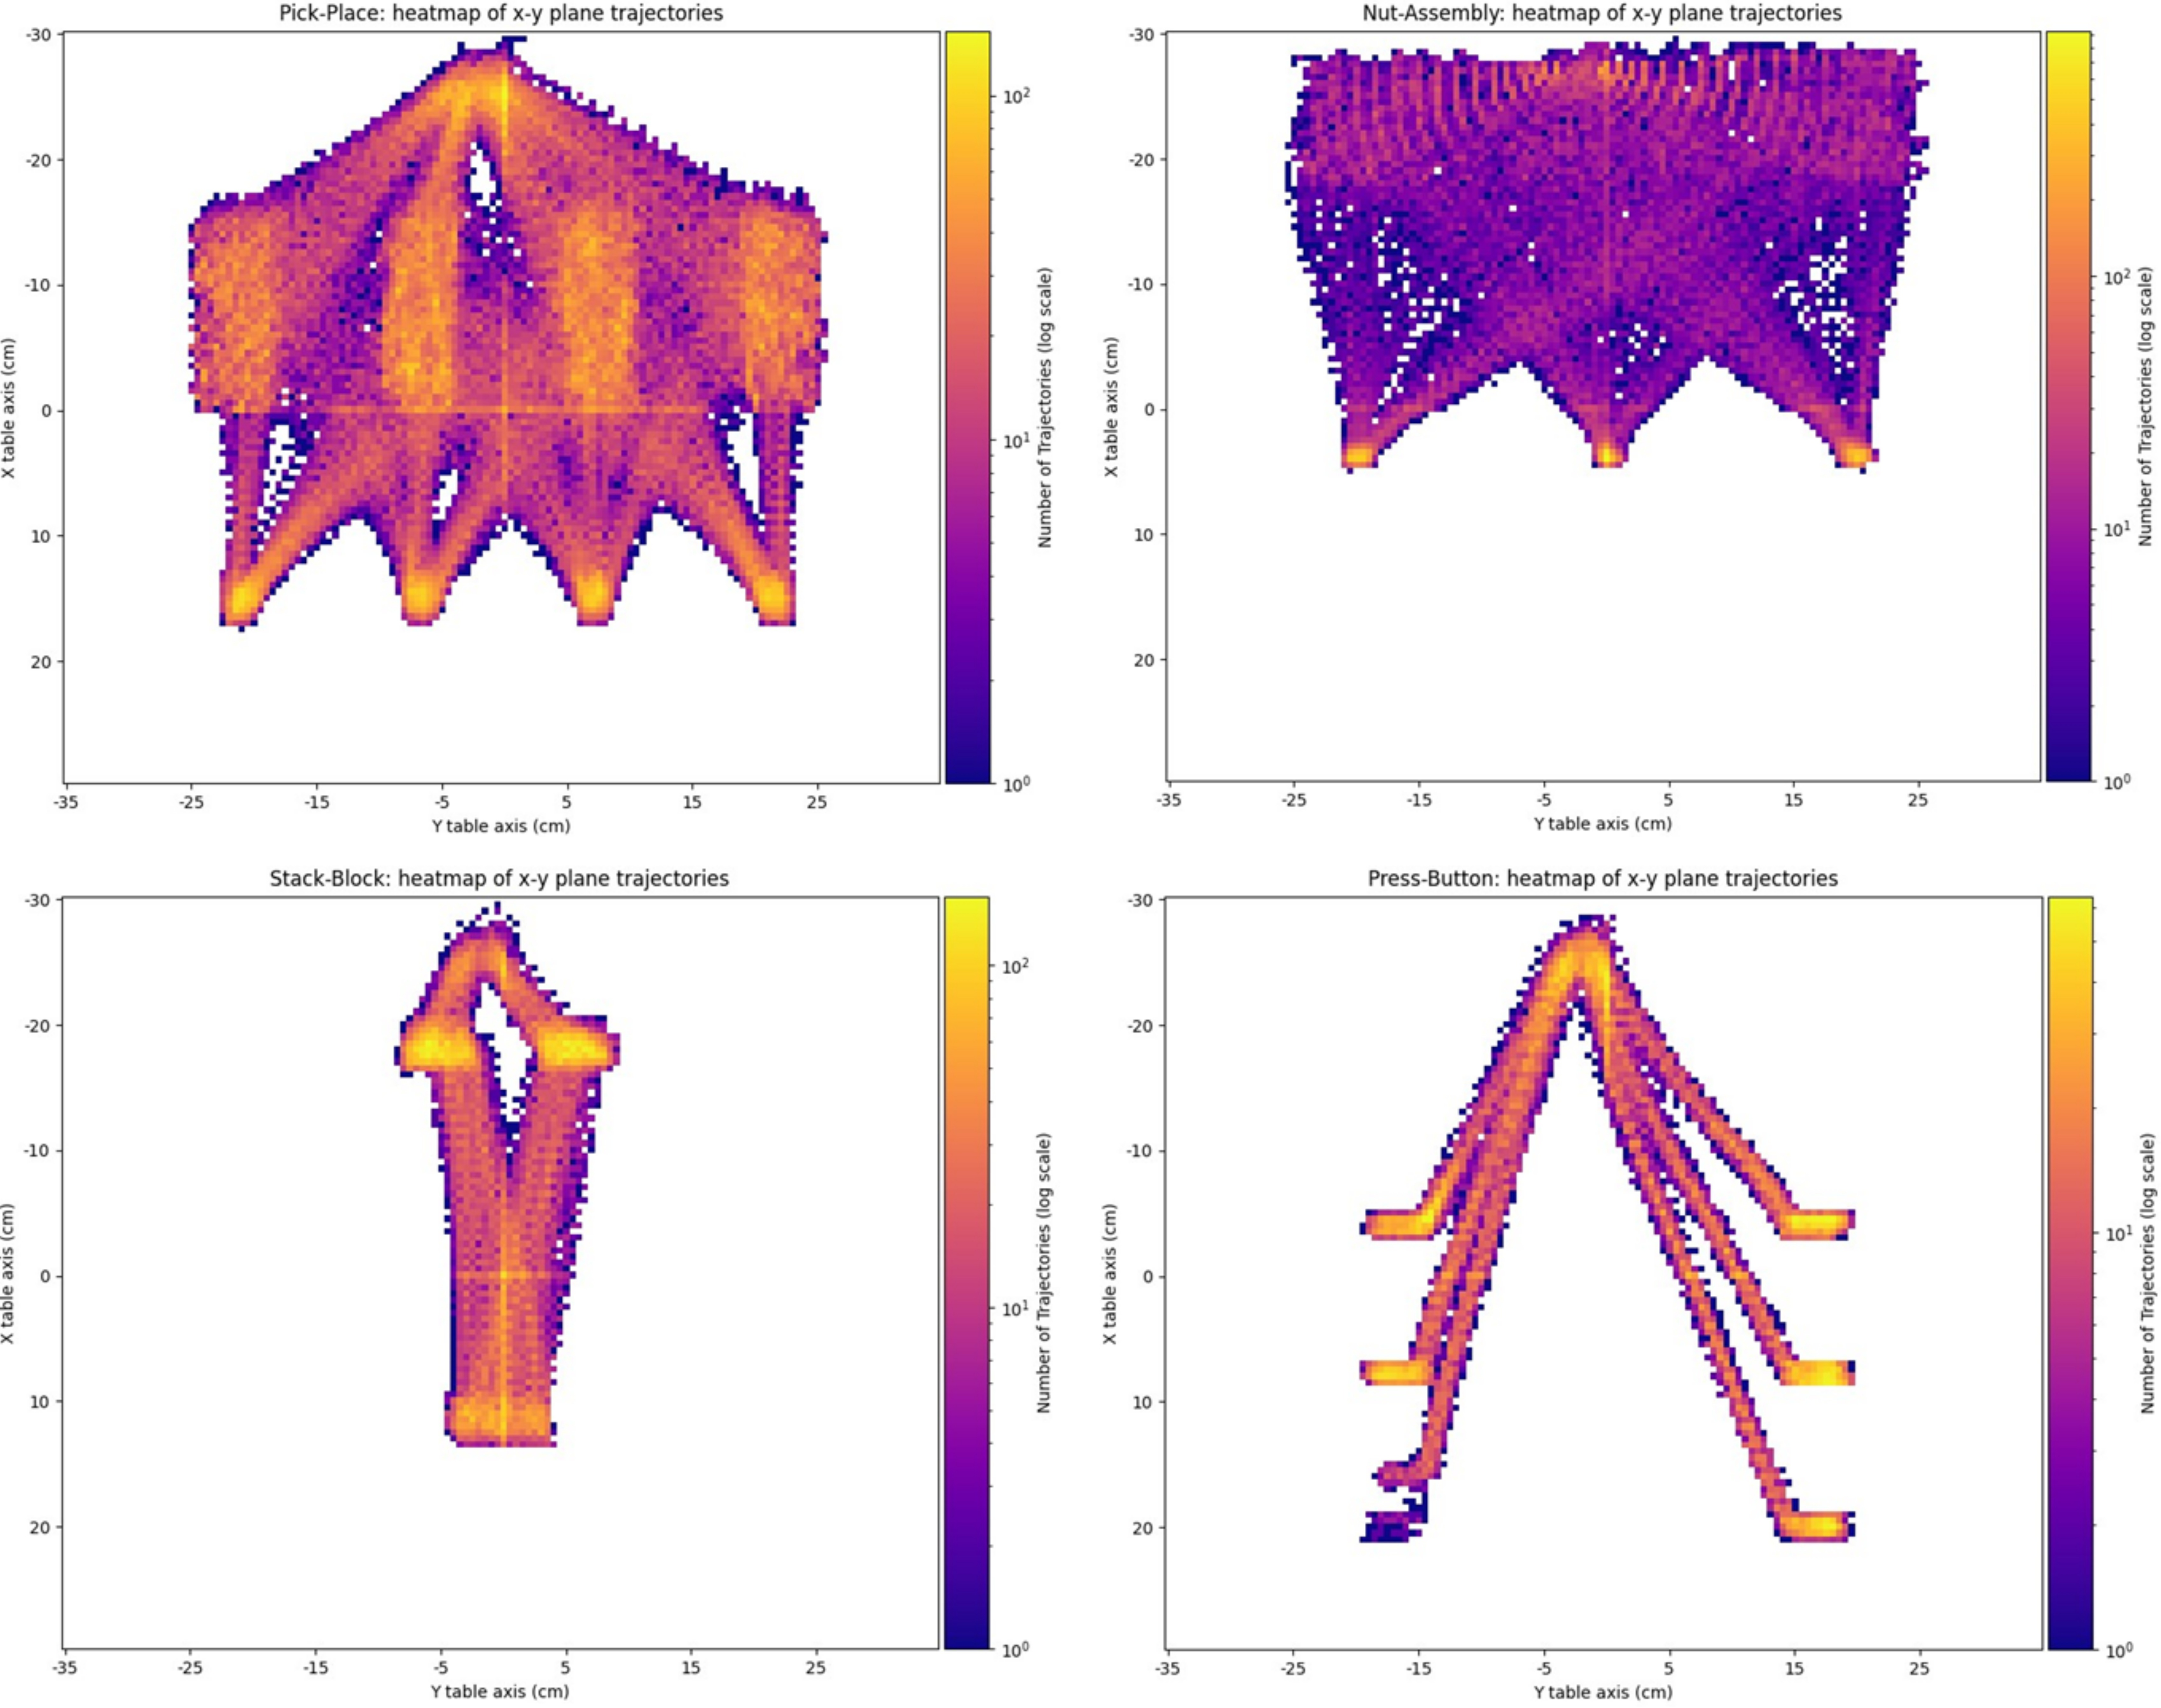
\includegraphics[width=1.0\textwidth]{figures/images/ch3/dataset_distribution.jpg}
    \caption{The distribution of trajectories for the different tasks along the x-y axis of the table workspace.}
    \label{fig:dataset_distribution}
\end{figure}

% The distribution of trajectories for the different tasks along the x-y axis of the table workspace. Each plot represents a density map illustrating the frequency with which the robot's end-effector passed through specific points across all variations and trajectories.
%  The tasks are organized as follows: (Top-Left) Pick-Place, (Top-Right) Nut-Assembly, (Bottom-Left) Stack-Block, and (Bottom-Right) Press-Button.

\subsection{Dataset}
\label{sec:ocpl_dataset}
The dataset used for training the control architectures is described in this section. It consists of the same tasks outlined in Section \ref{sec:cod_dataset}, following the same collection procedure. For each task variation, 100 trajectories were collected for both the agent and the demonstrator. Each trajectory presents a novel object configuration, according to the rules defined in Section \ref{sec:cod_dataset}.

In this section, the dataset is analyzed in terms of the distribution of the action space, in order to highlight the challenges from a control perspective.

Figure \ref{fig:dataset_distribution} illustrates the distribution of the trajectories followed by the robot. Each plot represents a density map illustrating the frequency with which the robot's end-effector passed through specific points across all variations and trajectories, specifically along the $x$ and $y$ axis. Notably, the use of a simulated environment enables complete coverage of the workspace. This particular aspect of the workspace coverage will be further discussed in Chapter \ref{ch:real_world_application} where the real-world system will be discussed.


% \smalltodo{Add figure here.}

Notably, each task exhibits a \textbf{multi-modal behavior}. This is evident across different variations, as the final placing position changes with each variation. Additionally, during the reaching phase, the robot traverses almost all possible locations within the working area.

It is important to note that, for a given task, the trajectories exhibit significant variation in length. Specifically, for the Pick-Place task, the average trajectory length is \textbf{$71.21 \pm 7.69$} frames. In the Nut-Assembly task, the average length is \textbf{$62.24 \pm 7.47$} frames, while for the Stack-Block task, the average is \textbf{$63.07 \pm 1.51$} frames. Finally, in the Press-Button task, the average trajectory length is\textbf{ $40.45 \pm 8.17$} frames. 

This variability poses a challenge, as the likelihood of errors increases with task progression, and compounding errors become more pronounced over time. Additionally, this multi-modal behavior complicates the learning process. The dataset lacks any prior distribution (i.e., the robot does not consistently approach the target object from the same direction), making it challenging for the architecture to identify and leverage consistent patterns during training.

\subsection{Results}
\label{sec:ocpl_results}
This section presents the obtained results, divided into two main blocks. The first block (Section~\ref{sec:ocpl_results_scm}) discusses the results of the method described in Section\ref{sec:ocpl_architecture_scm}. The second block (Section~\ref{sec:ocpl_results_dcm}) covers the results of the method described in \ref{sec:ocpl_architecture_dcm}. For each method, results are reported for two different scenarios: first, where the method is trained in a single-task multi-variation scenario; and second, where the method is trained in a multi-task multi-variation scenario.

The tests are conducted following the procedure outlined in Section \ref{sec:cod_results}. For each variation, 10 independent runs are performed, each with a novel initial objects configuration. This approach assesses the system robustness with respect to different initial state configurations. Additionally, each set of 10 rollouts is repeated three times to evaluate the overall robustness and consistency of the model.

Various evaluation metrics are considered, either generally defined for each task or task-specific. The general metrics include:

\begin{itemize}
    \item \textit{Reaching}: The ratio of successful attempts where the robot reaches the target object across all rollouts.
    \item \textit{Picking}: The ratio of successful attempts where the robot picks the correct object across all rollouts.
    \item \textit{Success}: The ratio of successful task completions across all rollouts.
    \item \textit{Reaching Wrong}: The ratio of instances where the robot reaches an object other than the target across all rollouts.
    \item \textit{Picking Wrong}: The ratio of instances where the robot picks the wrong object across all rollouts.
    \item \textit{Success with Wrong Object}: The ratio of task completions where the robot manipulates the wrong object.
\end{itemize}

Task-specific metrics, particularly for tasks like Pick-Place and Nut-Assembly, include the 
\textit{Place Wrong with Correct Object} metric, which captures the number of times the robot places the correct object in the wrong position.
% \begin{itemize}
%     \item \textit{Place Wrong with Wrong Object}: The number of times the robot completes the task by placing the wrong object in the wrong position.
%     \item \textit{Place Wrong with Correct Object}: The number of times the robot completes the task by placing the correct object in the wrong position.
% \end{itemize}

These metrics provide a comprehensive evaluation of the robot performance, capturing all major error cases and giving a full picture of its behavior.

\subsubsection{Single control module}
In this section the results obtained with the architecture composed of a Single Control Module will be described. As in Chapter \ref{ch:cod}, there are two testing scnearios, the first one trained with a single-task  multi-variation scenario, while the second one with a multi-task multi-variation setting, with an increasing level of complexity.
\label{sec:ocpl_results_scm}
\paragraph*{Single-task multi-variation scenario}\mbox{}\\

The discussion of the results begins with the single-task multi-variation scenario, focusing on the baseline methods TOSIL \cite{dasari2021transformers_one_shot} and MOSAIC \cite{mandi2022towards_more_generalizable_one_shot}. Specifically, Table \ref{table:occp_single_task_baseline_res} presents the performance of these baseline methods. 
% \usepackage{makecell}
% \usepackage{graphicx}
% \usepackage{multirow}
% \usepackage{hhline}


\begin{table}[t]
    \centering
    % \refstepcounter{table}
    \label{table:occp_single_task_baseline_res}
    \caption{The single-task performance of the baseline methods, TOSIL \cite{dasari2021transformers_one_shot} and MOSAIC \cite{mandi2022towards_more_generalizable_one_shot}, was evaluated. For each model, additional tests were conducted by generating the first 2 steps and 10 steps using the hand-written controller.}
    \resizebox{\linewidth}{!}{%
    \begin{tabular}{|c|c|c|c|c|c|c|c|c|} 
    \hline
    \textbf{Task} & \textbf{Model} & \textbf{GT Action} & \begin{tabular}[c]{@{}c@{}}\textbf{Reaching}\\{[}\%]\end{tabular} & \begin{tabular}[c]{@{}c@{}}\textbf{Picking}\\{[}\%]\end{tabular} & \begin{tabular}[c]{@{}c@{}}\textbf{Success}\\{[}\%]\end{tabular} & \begin{tabular}[c]{@{}c@{}}\textbf{Reaching} \\\textbf{Wrong}~\\{[}\%]\end{tabular} & \begin{tabular}[c]{@{}c@{}}\textbf{Picking}\\\textbf{Wrong}\\{[}\%]\end{tabular} & \begin{tabular}[c]{@{}c@{}}\textbf{Success with}\\\textbf{Wrong Object}\\{[}\%]\end{tabular} \\ 
    \hhline{|=========|}
    \multirow{6}{*}{\rotatebox[origin=c]{90}{Pick-Place}} & \multirow{3}{*}{MOSAIC} & 0 & 62.90$\pm$0.95 & 62.08$\pm$0.95 & 58.75$\pm$1.87 & 36.67$\pm$0.95 & 36.67$\pm$0.95 & \textbf{37.71$\pm$0.72} \\ 
    \cline{3-9}
     & & 2 & 89.17$\pm$1.30 & 88.12$\pm$
      0.62 & 84.17$\pm$
      1.57 & 11.25$\pm$
      1.25 & 11.25$\pm$
      1.25 & 11.46$\pm$
      1.30 \\ 
    \cline{3-9}
     &  & 10 & 99.79$\pm$0.36 & 98.54$\pm$0.72 & \textbf{95.63$\pm$0.63} & 1.25$\pm$0.63 & 1.25$\pm$0.63 & 0.41$\pm$0.36 \\ 
    \cline{2-9}
     & \multirow{3}{*}{TOSIL} & 0 & 33.12$\pm$1.08 & 27.92$\pm$
      0.72 & 26.87$\pm$
      0.62 & 63.96$\pm$
      2.36 & 63.75$\pm$
      2.72 & \textbf{66.04$\pm$1.57} \\ 
    \cline{3-9}
     & & 2 & 69.17$\pm$1.30 & 60.83$\pm$2.52 & 59.38$\pm$2.17 & 29.17$\pm$0.95 & 28.96$\pm$1.30 & 30.83$\pm$2.20 \\ 
    \cline{3-9}
     &  & 10 & 98.58$\pm$0.36 & 92.71$\pm$
      1.44 & \textbf{90.00$\pm$1.08} & 2.70$\pm$
      1.30 & 2.70$\pm$
      1.30 & 1.25$\pm$
      0.62 \\ 
    \hhline{|=========|}
    \multirow{6}{*}{\rotatebox[origin=c]{90}{Nut-Assembly}} & \multirow{3}{*}{MOSAIC} & 0 & 38.89$\pm$1.11 & 36.67$\pm$1.11 & 33.33$\pm$1.11 & 59.26$\pm$1.69 & 55.93$\pm$1.69 & \textbf{51.48$\pm$2.31} \\ 
    \cline{3-9}
     & & 2 & 85.19$\pm$
      4.49 & 83.33$\pm$
      5.09 & 78.89$\pm$
      4.01 & 13.33$\pm$
      4.84 & 11.85$\pm$
      2.31 & 11.11$\pm$
      2.22 \\ 
    \cline{3-9}
     &  & 10 & 100.00$\pm$100.00 & 99.26$\pm$1.28 & \textbf{90.74$\pm$2.79} & 0.00$\pm$0.00 & 0.00$\pm$0.00 & 0.00$\pm$0.00 \\ 
    \cline{2-9}
     & \multirow{3}{*}{TOSIL} & 0 & 36.30$\pm$
      1.28 & 35.19$\pm$
      2.31 & 31.11$\pm$
      1.92 & 63.33$\pm$
      1.11 & 62.59$\pm$
      1.28 & \textbf{56.30$\pm$3.57} \\ 
    \cline{3-9}
     & & 2 & 83.33$\pm$2.22 & 82.96$\pm$2.31 & 77.78$\pm$2.22 & 16.67$\pm$2.22 & 16.67$\pm$2.22 & 14.44$\pm$1.11 \\ 
    \cline{3-9}
     &  & 10 & 100.00$\pm$
      0.00 & 99.26$\pm$
      1.28 & \textbf{88.89$\pm$2.22} & 0.00$\pm$
      0.00 & 0.00$\pm$
      0.00 & 0.00$\pm$
      0.00 \\ 
    \hhline{|=========|}
    \multirow{6}{*}{\rotatebox[origin=c]{90}{Stack-Block}} & \multirow{3}{*}{MOSAIC} & 0 & 60.56$\pm$0.96 & 60.56$\pm$0.96 & 53.33$\pm$1.66 & 39.44$\pm$0.96 & 39.44$\pm$0.96 & \textbf{36.11$\pm$0.96} \\ 
    \cline{3-9}
     & & 2 & 91.11$\pm$
      0.96 & 90.56$\pm$
      0.96 & 73.89$\pm$
      4.19 & 7.70$\pm$
      0.96 & 7.70$\pm$
      0.96 & 7.20$\pm$
      0.96 \\ 
    \cline{3-9}
     &  & 10 & 100.00$\pm$0.00 & 99.44$\pm$0.96 & \textbf{77.78$\pm$1.92} & 0.00$\pm$0.00 & 0.00$\pm$0.00 & 0.00$\pm$0.00 \\ 
    \cline{2-9}
     & \multirow{3}{*}{TOSIL} & 0 & 69.44$\pm$
      0.96 & 60.00$\pm$
      0.16 & 48.89$\pm$
      2.54 & 42.78$\pm$
      0.96 & 42.78$\pm$
      0.96 & \textbf{41.67$\pm$1.66} \\ 
    \cline{3-9}
     & & 2 & 90.56$\pm$0.96 & 87.78$\pm$0.96 & 79.44$\pm$1.92 & 12.22$\pm$0.96 & 11.67$\pm$0.00 & 11.67$\pm$0.00 \\ 
    \cline{3-9}
     &  & 10 & 100.00$\pm$
      0.00 & 99.44$\pm$
      0.96 & \textbf{88.89$\pm$1.92} & 1.66$\pm$
      1.66 & 1.11$\pm$
      0.96 & 0.00$\pm$
      0.00 \\ 
    \hhline{|=========|}
    \multirow{6}{*}{\rotatebox[origin=c]{90}{Press-Button}} & \multirow{3}{*}{MOSAIC} & 0 & 100.00$\pm$0.00 & - & \textbf{100.00$\pm$0.00} & 0.00$\pm$0.00 & - & 0.00$\pm$0.00 \\ 
    \cline{3-9}
     & & 2 & 100.00$\pm$
      0.00 & - & 100.00,
      0.00 & 0.00$\pm$
      0.00 & - & 0.00$\pm$
      0.00 \\ 
    \cline{3-9}
     &  & 10 & 100.00$\pm$0.00 & - & 100.00$\pm$0.00 & 0.00$\pm$0.00 & - & 0.00$\pm$0.00 \\ 
    \cline{2-9}
     & \multirow{3}{*}{TOSIL} & 0 & 83.33$\pm$
      1.66 & - & \textbf{83.33$\pm$1.66} & 17.78$\pm$
      1.93 & - & 16.67$\pm$
      1.67 \\ 
    \cline{3-9}
     & & 2 & 80.56$\pm$1.92 & - & 80.56$\pm$1.92 & 20.00$\pm$2.88 & - & 18.33$\pm$2.89 \\ 
    \cline{3-9}
     &  & 10 & 92.22$\pm$
      0.96 & - & 81.67$\pm$
      3.33 & 9.44$\pm$
      0.96 & - & 9.44$\pm$
      0.96 \\
    \hline
    \end{tabular}
    }
    \end{table}

As observed, both baseline methods suffer from the issue of \textbf{target-object misidentification}. This is evident from the \textit{Success with Wrong Object} column, where the success rate involving wrong objects is significant. Figure \ref{fig:baseline_pick_place_error} provides an example of a pick-and-place rollout in which the task is technically completed, but the wrong object is manipulated.
\begin{figure}[t]
    \centering
    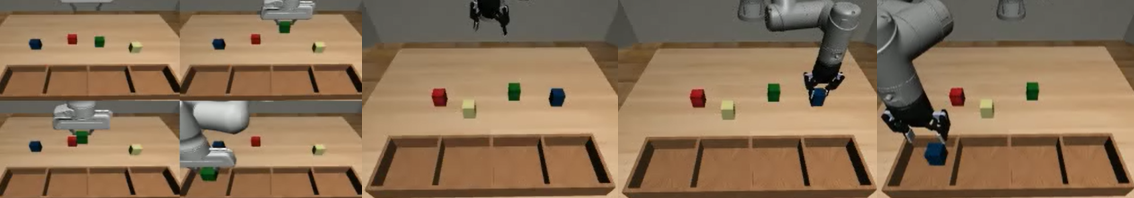
\includegraphics[width=1.0\textwidth]{figures/images/baseline_pick_place_error/pick_place_trj.png}
    \caption{Example of task rollout with incorrect object manipulation. In this scenario, the robot successfully completes the task by placing an object in the first bin. However, instead of manipulating the correct object (the green box), the robot mistakenly picks up the blue box. This illustrates a situation where the robot executes the task's final action correctly but selects the wrong object during manipulation.}
    \label{fig:baseline_pick_place_error}
\end{figure}

% \smalltodo{Add Figure}

To investigate the cause of these errors, test rollouts were performed using the first 2 and 10 actions generated by a hand-written policy, which has access to ground-state information. As noted, the success rate improves substantially by applying just 2 ground-truth actions. This supports the hypothesis outlined in Section \ref{sec:ocpl_problem}, suggesting that the end-to-end architecture trained with an action-centric loss produces a suboptimal embedding $z$ for the cognitive task. The embedding fails to sufficiently inform the control policy about the correct position of the target object.

Based on this consideration, the thesis proposal to inform the control module with both a low-level positional information (e.g., the bouding-box of the target object) and a control embedding generated by the MOSAIC-backbone has been tested. During this test, two models variations have been considered, the first named \textit{MOSAIC-GT-BB} is basically the MOSAIC model, with the Control Module that receives in input the control-embedding $z^{control}$ and the ground-truth bouding-box. The second, named \textit{MOSAIC-CTOD} is the architecture described in Section \ref{sec:ocpl_architecture_scm}.

\begin{table}[t]
  \centering
  \caption{The single-task performance of the proposed MOSAIC-CTOD module is compared to the MOSAIC and MOSAIC-GT-BB baselines. MOSAIC-GT-BB refers to the MOSAIC model, where the Control Module receives the ground-truth target bounding box as input.}
  \label{table:ctod_single_task}
  \resizebox{\linewidth}{!}{%
  \begin{tabular}{|c|c|c|c|c|c|c|c|} 
  \hline
  \textbf{Task} & \textbf{Method} & \begin{tabular}[c]{@{}c@{}}\textbf{Reaching}\\{[}\%]\end{tabular} & \begin{tabular}[c]{@{}c@{}}\textbf{Picking}\\{[}\%]\end{tabular} & \begin{tabular}[c]{@{}c@{}}\textbf{Success}\\{[}\%]\end{tabular} & \begin{tabular}[c]{@{}c@{}}\textbf{Reaching }\\\textbf{Wrong~}\\{[}\%]\end{tabular} & \begin{tabular}[c]{@{}c@{}}\textbf{Picking}\\\textbf{Wrong}\\{[}\%]\end{tabular} & \begin{tabular}[c]{@{}c@{}}\textbf{Success with}\\\textbf{Wrong Object}\\{[}\%]\end{tabular} \\ 
  \hhline{|========|}
  \multirow{3}{*}{Pick-Place} & MOSAIC & 62.90$\pm$0.95 & 62.08$\pm$0.95 & 58.75$\pm$1.87 & 36.67$\pm$0.95 & 36.67$\pm$0.95 & 37.71$\pm$0.72 \\ 
  \cline{2-8}
   & MOSAIC-GT-BB & 100.00$\pm$   0.00 & 97.71$\pm$   0.72 & 76.46$\pm$   3.20 & 0.00$\pm$   0.00 & 0.00$\pm$   0.00 & 0.00$\pm$   0.00 \\ 
  \cline{2-8}
   & MOSAIC-CTOD & 98.12$\pm$0.62 & 91.88$\pm$4.88 & \textbf{77.11$\pm$5.60} & 1.04$\pm$0.36 & 1.04$\pm$0.36 & 1.04$\pm$0.36 \\ 
  \hhline{|========|}
  \multirow{3}{*}{Nut-Assembly} & MOSAIC & 38.89$\pm$1.11 & 36.67$\pm$1.11 & 33.33$\pm$1.11 & 59.26$\pm$1.69 & 55.93$\pm$1.69 & 51.48$\pm$2.31 \\ 
  \cline{2-8}
   & MOSAIC-GT-BB & 100.00$\pm$   0.00 & 98.89$\pm$   1.11 & \textbf{70.37$\pm$1.69} & 0.00$\pm$   0.00 & 0.00$\pm$   0.00 & 0.00$\pm$   0.00 \\ 
  \cline{2-8}
   & MOSAIC-CTOD & 98.89$\pm$1.11 & 97.41$\pm$2.31 & 64.07$\pm$0.64 & 0.00$\pm$0.00 & 0.00$\pm$0.00 & 0.00$\pm$0.00 \\ 
  \hhline{|========|}
  \multirow{3}{*}{Stack-Block} & MOSAIC & 60.56$\pm$0.96 & 60.56$\pm$0.96 & 53.33$\pm$1.66 & 39.44$\pm$0.96 & 39.44$\pm$0.96 & 36.11$\pm$0.96 \\ 
  \cline{2-8}
   & MOSAIC-GT-BB & 100.00$\pm$   0.00 & 99.44$\pm$   0.96 & 90.00$\pm$   2.89 & 0.00$\pm$   0.00 & 0.00$\pm$   0.00 & 0.00$\pm$   0.00 \\ 
  \cline{2-8}
   & MOSAIC-CTOD & 100.00$\pm$0.00 & 100.00$\pm$0.00 & \textbf{91.67$\pm$2.88} & 0.00$\pm$0.00 & 0.00$\pm$0.00 & 0.00$\pm$0.00 \\ 
  \hhline{|========|}
  \multirow{3}{*}{Press-Button} & MOSAIC & 100.00$\pm$0.00 & - & \textbf{100.00$\pm$0.00} & 0.00$\pm$0.00 & - & 0.00$\pm$0.00 \\ 
  \cline{2-8}
   & MOSAIC-GT-BB & 92.22$\pm$   2.54 & - & 90.56$\pm$   1.92 & 3.88$\pm$   0.96 & - & 3.88$\pm$   0.96 \\ 
  \cline{2-8}
   & MOSAIC-CTOD & 97.22$\pm$1.92 & - & 95.56$\pm$1.92 & 2.77$\pm$0.96 & - & 2.77$\pm$0.96 \\
  \hline
  \end{tabular}
  }
  \end{table}
The results are summarized in Table \ref{table:ctod_single_task_performance}. Several key observations can be made from these findings. For tasks involving multiple similar objects that change positions across different demonstrations (such as Pick-Place, Nut-Assembly, and Stack-Block), the use of positional information significantly enhances the system robustness. This enables the robot to consistently reach the target object and improves the overall success rate.

In contrast, for the Press-Button task, although the MOSAIC-CTOD method achieves a high success rate (95.56\% on average), it does not overcome the baseline method, which consistently solves the task with a 100\% success rate. This is because, once the button is reached, the positional information does not provide any additional guidance on how to complete the task. As a result, the robot tends to get stuck near the button, failing to execute the pushing action (Figure \ref{fig:button_ctod_error}).
\begin{figure}[t]
    \centering
    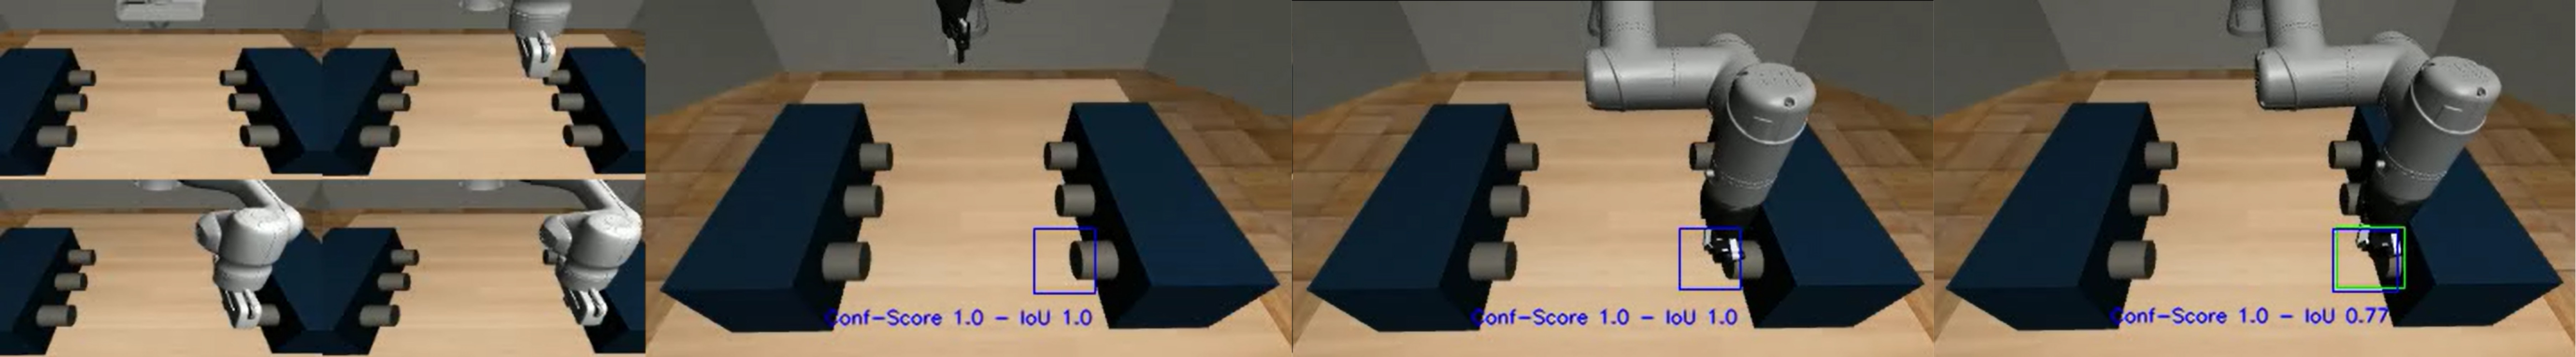
\includegraphics[width=1.0\textwidth]{figures/images/ch3/button_error.jpg}
    \caption{Example of unsuccessful Press-Button rollout. In this scenario, the robot successfully reaches the target button using the predicted bounding box (blue). However, due to instability in predictions during the pushing phase, the robot is unable to complete the pressing action, resulting in an unsuccessful task execution.}
    \label{fig:button_ctod_error}
\end{figure}

% \smalltodo{Add Figure}

Furthermore, the inclusion of positional information introduces a novel type of error. Specifically, since the robot behavior is conditioned by the bounding box, any error in its prediction can cause the robot to move incorrectly (Figure \ref{fig:error_propagation}). This error is significant, as in the Pick-Place task, the metric ``Place Wrong with Correct Object" reaches 11.25\%, and for the Nut-Assembly task, the same metric averages 22.22\%.
\begin{figure}[t]
    \centering
    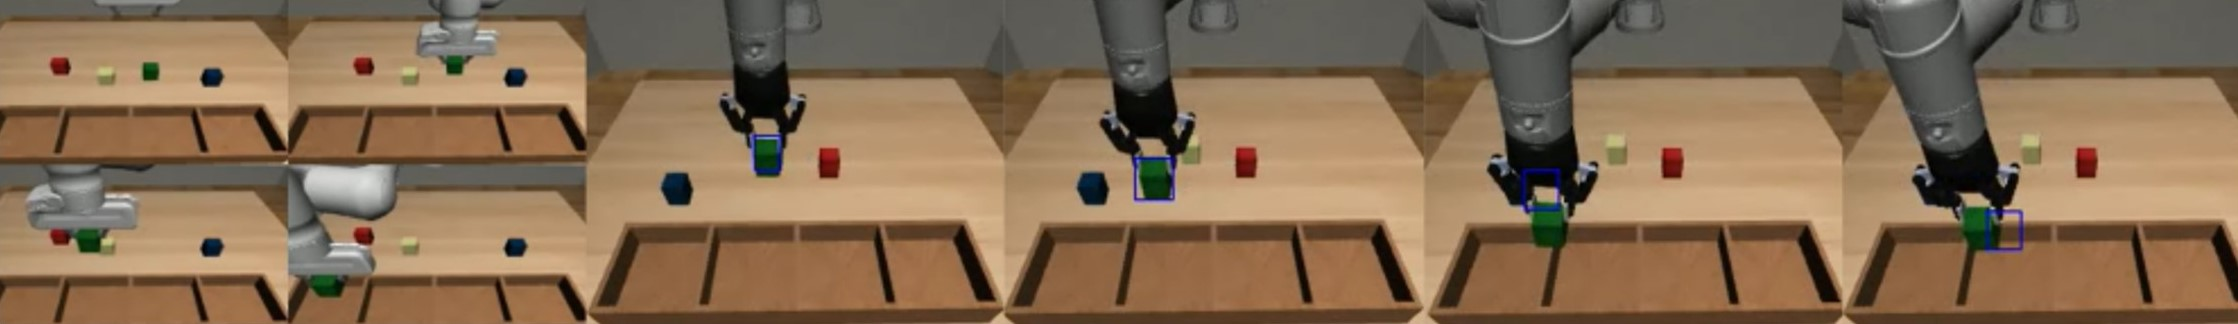
\includegraphics[width=1.0\textwidth]{figures/images/ch3/error_propagation.jpg}
    \caption{Example of unsuccessful Pick-Place rollout. In this case, the robot fails to complete the task due to errors in the bounding box predictions. These inaccuracies cause the robot to move in the wrong direction, leading to an unsuccessful execution of the task.}
    \label{fig:error_propagation}
\end{figure}


To address this issue, the Double-Control Module architecture has been proposed (Section \ref{sec:ocpl_architecture_dcm}), with the corresponding results presented in Section \ref{sec:ocpl_results_dcm}.

\paragraph*{Multi-task multi-variation scenario}\mbox{}\\
As in the previous paragraph, an evaluation of the two baseline methods was also conducted in the multi-task setting. The results are summarized in Table \ref{table:occp_multi_task_baseline_res}. The same general trends and behaviors observed in the single-task scenario are present here as well. Specifically, both baselines demonstrate the ability to produce reasonable trajectories that allow the robot to complete the task, though they manipulate the wrong object.

Furthermore, when comparing the results from Table \ref{table:occp_single_task_baseline_res} with those in Table \ref{table:occp_multi_task_baseline_res}, it is evident that the success rate decreases across all methods in the more complex multi-task setting. This highlights a potential issue with task balancing during the learning process.
% \usepackage{makecell}
% \usepackage{graphicx}
% \usepackage{multirow}
% \usepackage{hhline}


\begin{table}[t]
  \centering
  \caption{The multi-task performance of the baseline methods, TOSIL \cite{dasari2021transformers_one_shot} and MOSAIC \cite{mandi2022towards_more_generalizable_one_shot}, was evaluated. For each model, additional tests were conducted by generating the first 2 steps and 10 steps using the hand-written controller.}
  \label{table:occp_multi_task_baseline_res}
  \resizebox{\linewidth}{!}{%
  \begin{tabular}{|c|c|c|c|c|c|c|c|c|} 
  \hline
  \textbf{Task} & \textbf{Model} & \textbf{GT Action} & \begin{tabular}[c]{@{}c@{}}\textbf{Reaching}\\{[}\%]\end{tabular} & \begin{tabular}[c]{@{}c@{}}\textbf{Picking}\\{[}\%]\end{tabular} & \begin{tabular}[c]{@{}c@{}}\textbf{Success}\\{[}\%]\end{tabular} & \begin{tabular}[c]{@{}c@{}}\textbf{Reaching} \\\textbf{Wrong}~\\{[}\%]\end{tabular} & \begin{tabular}[c]{@{}c@{}}\textbf{Picking}\\\textbf{Wrong}\\{[}\%]\end{tabular} & \begin{tabular}[c]{@{}c@{}}\textbf{Success with}\\\textbf{Wrong Object}\\{[}\%]\end{tabular} \\ 
  \hhline{|=========|}
  \multirow{6}{*}{\rotatebox[origin=c]{90}{Pick-Place}} & \multirow{3}{*}{MOSAIC} & 0 & 25.83$\pm$1.30 & 23.96$\pm$0.72 & 22.71$\pm$0.72 & 65.63$\pm$2.87 & 63.96$\pm$1.90 & \textbf{67.92$\pm$1.30} \\ 
  \cline{3-9}
   &  & 2 & 61.04$\pm$2.19 & 58.13$\pm$2.86 & 56.46$\pm$3.14 & 36.04$\pm$1.90 & 35.42$\pm$1.90 & 36.25$\pm$1.08 \\ 
  \cline{3-9}
   &  & 10 & 97.77$\pm$0.36 & 95.00$\pm$0.62 & \textbf{87.50$\pm$1.25} & 2.50$\pm$0.62 & 2.29$\pm$0.95 & 2.29$\pm$0.72 \\ 
  \cline{2-9}
   & \multirow{3}{*}{TOSIL} & 0 & 35.42$\pm$0.72 & 27.08$\pm$1.30 & 26.46$\pm$1.80 & 60.21$\pm$1.57 & 59.58$\pm$1.44 & 59.58$\pm$1.44 \\ 
  \cline{3-9}
   &  & 2 &  &  &  &  &  &  \\ 
  \cline{3-9}
   &  & 10 &  &  &  &  &  &  \\ 
  \hhline{|=========|}
  \multirow{6}{*}{\rotatebox[origin=c]{90}{Stack-Block}} & \multirow{3}{*}{MOSAIC} & 0 & 32.96$\pm$1.28 & 30.74$\pm$2.31 & 28.53$\pm$2.31 & 56.30$\pm$4.49 & 48.15$\pm$4.20 & 41.67$\pm$1.66 \\ 
  \cline{3-9}
   &  & 2 & 76.67$\pm$1.11 & 73.33$\pm$1.92 & 65.56$\pm$4.00 & 19.63$\pm$0.64 & 17.41$\pm$1.28 & 17.04$\pm$1.69 \\ 
  \cline{3-9}
   &  & 10 & 100.00$\pm$0.00 & 97.78$\pm$1.11 & \textbf{82.96$\pm$1.28} & 0.00$\pm$0.00 & 0.00$\pm$0.00 & 0.00$\pm$0.00 \\ 
  \cline{2-9}
   & \multirow{3}{*}{TOSIL} & 0 & 27.78$\pm$2.94 & 24.44$\pm$2.94 & 22.59$\pm$3.57 & 70.37$\pm$2.57 & 67.78$\pm$2.22 & \textbf{64.81$\pm$2.57} \\ 
  \cline{3-9}
   &  & 2 &  &  &  &  &  &  \\ 
  \cline{3-9}
   &  & 10 &  &  &  &  &  &  \\ 
  \hhline{|=========|}
  \multirow{6}{*}{\rotatebox[origin=c]{90}{Nut-Assembly}} & \multirow{3}{*}{MOSAIC} & 0 & 57.78$\pm$1.92 & 57.78$\pm$1.92 & 55.56$\pm$2.54 & 42.22$\pm$1.92 & 42.22$\pm$1.93 & 41.11$\pm$1.67 \\ 
  \cline{3-9}
   &  & 2 & 95.56$\pm$0.96 & 95.56$\pm$0.96 & 89.44$\pm$1.92 & 4.44$\pm$0.96 & 4.44$\pm$0.96 & 4.44$\pm$0.96 \\ 
  \cline{3-9}
   &  & 10 & 100.00$\pm$0.00 & 100.00$\pm$0.00 & \textbf{92.22$\pm$0.96} & 0.00$\pm$0.00 & 0.00$\pm$0.00 & 0.00$\pm$0.00 \\ 
  \cline{2-9}
   & \multirow{3}{*}{TOSIL} & 0 & 54.44$\pm$0.96 & 54.44$\pm$0.96 & 48.89$\pm$0.96 & 46.11$\pm$0.96 & 45.56$\pm$0.96 & \textbf{45.56$\pm$0.96} \\ 
  \cline{3-9}
   &  & 2 &  &  &  &  &  &  \\ 
  \cline{3-9}
   &  & 10 &  &  &  &  &  &  \\ 
  \hhline{|=========|}
  \multirow{6}{*}{\rotatebox[origin=c]{90}{Press-Button}} & \multirow{3}{*}{MOSAIC} & 0 & 78.33$\pm$1.66 & - & 77.22$\pm$2.54 & 22.78$\pm$2.54 & - & 22.78$\pm$2.54 \\ 
  \cline{3-9}
   &  & 2 & 77.22$\pm$0.96 & - & 76.67$\pm$1.67 & 23.33$\pm$1.66 & - & 23.33$\pm$1.66 \\ 
  \cline{3-9}
   &  & 10 & 82.78$\pm$2.54 & - & \textbf{80.00$\pm$3.33} & 20.00$\pm$3.33 & - & 20.00$\pm$3.33 \\ 
  \cline{2-9}
   & \multirow{3}{*}{TOSIL} & 0 & 70.56$\pm$7.52 & - & 60.59$\pm$11.34 & 27.22$\pm$2.47 & - & \textbf{27.22$\pm$2.47} \\ 
  \cline{3-9}
   &  & 2 &  & - &  &  & - &  \\ 
  \cline{3-9}
   &  & 10 &  & - &  &  & - &  \\
  \hline
  \end{tabular}
  }
  \end{table}

After evaluating the baseline, the proposed MOSAIC-CTOD was tested, using the same variations as in the previous section. Table \ref{table:ctod_multi_task} summarizes the results obtained with the inclusion of positional information. Compared to the baseline, a general improvement is observed. However, caution is required when training the system in a multi-task setting. Specifically, when comparing the single-task performance (Table \ref{table:mosaic_ctod_single_task}) to the multi-task performance, there is a noticeable drop in success rates for the same tasks. This decline is particularly evident in the system's ability to execute the ``pick" primitive, especially when the nut object is involved. This observation underscores the importance of incorporating regularization techniques during multi-task learning to manage the varying complexities of different tasks.
% \usepackage{graphicx}
% \usepackage{multirow}
% \usepackage{hhline}


\begin{table}[t]
  \centering
  \caption{The multi-task performance of the proposed MOSAIC-CTOD module is compared to the MOSAIC and MOSAIC-GT-BB baselines. MOSAIC-GT-BB refers to the MOSAIC model, where the Control Module receives the ground-truth target bounding box as input.}
  \label{table:ctod_multi_task}
  \resizebox{\linewidth}{!}{%
  \begin{tabular}{|c|c|c|c|c|c|c|c|} 
  \hline
  \textbf{Task} & \textbf{Method} & \begin{tabular}[c]{@{}c@{}}\textbf{Reaching}\\{[}\%]\end{tabular} & \begin{tabular}[c]{@{}c@{}}\textbf{Picking}\\{[}\%]\end{tabular} & \begin{tabular}[c]{@{}c@{}}\textbf{Success}\\{[}\%]\end{tabular} & \begin{tabular}[c]{@{}c@{}}\textbf{Reaching }\\\textbf{Wrong~}\\{[}\%]\end{tabular} & \begin{tabular}[c]{@{}c@{}}\textbf{Picking}\\\textbf{Wrong}\\{[}\%]\end{tabular} & \begin{tabular}[c]{@{}c@{}}\textbf{Success with}\\\textbf{Wrong Object}\\{[}\%]\end{tabular} \\ 
  \hhline{|========|}
  \multirow{3}{*}{Pick-Place} & MOSAIC & 25.83$\pm$1.30 & 23.96$\pm$0.72 & 22.71$\pm$0.72 & 65.63$\pm$2.87 & 63.96$\pm$1.90 & 67.92$\pm$1.30 \\ 
  \cline{2-8}
   & MOSAIC-GT-BB & 100.00$\pm$0.00 & 89.58$\pm$2.19 & \textbf{58.33$\pm$0.90} & 0.00$\pm$0.00 & 0.00$\pm$0.00 & 0.00$\pm$0.00 \\ 
  \cline{2-8}
   & \begin{tabular}[c]{@{}c@{}}\textit{\textbf{MOSAIC-CTOD}}\\\textit{\textbf{(proposal)}}\end{tabular} & 80.21$\pm$1.44 & 67.50$\pm$0.62 & 53.33$\pm$1.90 & 4.16$\pm$0.71 & 3.54$\pm$0.36 & 0.37$\pm$0.64 \\ 
  \hhline{|========|}
  \multirow{3}{*}{Nut-Assembly} & MOSAIC & 32.96$\pm$1.28 & 30.74$\pm$2.31 & 28.53$\pm$2.31 & 56.30$\pm$4.49 & 48.15$\pm$4.20 & 41.67$\pm$1.66 \\ 
  \cline{2-8}
   & MOSAIC-GT-BB & 99.63$\pm$0.64 & 91.48$\pm$2.31 & \textbf{37.04$\pm$5.70} & 0.00$\pm$0.00 & 0.00$\pm$0.00 & 0.00$\pm$0.00 \\ 
  \cline{2-8}
   & \begin{tabular}[c]{@{}c@{}}\textit{\textbf{MOSAIC-CTOD}}\\\textit{\textbf{(proposal)}}\end{tabular} & 68.69$\pm$1.11 & 49.63$\pm$3.30 & 33.33$\pm$4.00 & 11.48$\pm$1.69 & 5.55$\pm$2.94 & 0.00$\pm$0.00 \\ 
  \hhline{|========|}
  \multirow{3}{*}{Stack-Block} & MOSAIC & 57.78$\pm$1.92 & 57.78$\pm$1.92 & 55.56$\pm$2.54 & 42.22$\pm$1.92 & 42.22$\pm$1.93 & 41.11$\pm$1.67 \\ 
  \cline{2-8}
   & MOSAIC-GT-BB & 94.44$\pm$5.85 & 91.11$\pm$6.73 & 73.89$\pm$5.00 & 10.00$\pm$2.88 & 0.00$\pm$0.00 & 0.00$\pm$0.00 \\ 
  \cline{2-8}
   & \begin{tabular}[c]{@{}c@{}}\textit{\textbf{MOSAIC-CTOD}}\\\textit{\textbf{(proposal)}}\end{tabular} & 97.92$\pm$2.09 & 96.67$\pm$2.35 & \textbf{87.92$\pm$2.00} & 1.25$\pm$0.83 & 0.41$\pm$0.83 & 0.00$\pm$0.00 \\ 
  \hhline{|========|}
  \multirow{3}{*}{Press-Button} & MOSAIC & 78.33$\pm$1.66 & - & 77.22$\pm$2.54 & 22.78$\pm$2.54 & - & 22.78$\pm$2.54 \\ 
  \cline{2-8}
   & MOSAIC-GT-BB & 100.00$\pm$0.00 & - & \textbf{98.33$\pm$0.00} & 0.55$\pm$0.96 & - & 0.55$\pm$0.96 \\ 
  \cline{2-8}
   & \begin{tabular}[c]{@{}c@{}}\textbf{\textit{MOSAIC-CTOD}}\\\textbf{\textit{(proposal)}}\end{tabular} & 92.78$\pm$0.96 & - & 91.11$\pm$2.54 & 3.89$\pm$4.19 & - & 3.88$\pm$4.19 \\
  \hline
  \end{tabular}
  }
  \end{table}

\subsubsection{Double control modules}
In this section the results obtained with the Double Control Module (Section \ref{sec:ocpl_architecture_dcm}) are going to be discussed.
\label{sec:ocpl_results_dcm}
\paragraph*{Single-task multi-variation scenario}\mbox{}\\
As discussed in Section \ref{sec:ocpl_architecture_dcm}, the introduction of the Double Control Module (DCM) was motivated by the need to reduce errors associated with incorrect object placement. These errors arise from inaccurate bounding-box predictions, which can lead to error propagation. 

To address this issue, the architecture of the Double Control Module evolved through incremental design iterations and validation steps.
Specifically, the process started by observing that the positional information given by the bouding-box is useful only during the reaching phase, while it becomes useless after it. For this reason, the training of the MOSAIC-CTOD has been changed, setting to zero the bounding-box after the picking. Then, observing the obtained results and the error cases, the Double Control Module has been realized.

% \usepackage{graphicx}
% \usepackage{multirow}
% \usepackage{hhline}


\begin{table}[t]
  \centering
  \caption{MOSAIC-COD results obtained in the single-task setting. The model is compared to baselines such as MOSAIC-CTOD (Section \ref{sec:ocpl_results_scm}), a modified version of MOSAIC-CTOD that does not receive the predicted bounding box after picking, and MOSAIC-DP, which is the MOSAIC architecture proposed in \cite{mandi2022towards_more_generalizable_one_shot}, but with two control modules.}
  \label{table:double_policy_single_task}
  \resizebox{\linewidth}{!}{%
  \begin{tabular}{|c|c|c|c|c|c|} 
  \hline
  \textbf{Task} & \textbf{Model} & \begin{tabular}[c]{@{}c@{}}\textbf{Reaching}\\{[}\%]\end{tabular} & \begin{tabular}[c]{@{}c@{}}\textbf{Picking}\\{[}\%]\end{tabular} & \begin{tabular}[c]{@{}c@{}}\textbf{Success}\\{[}\%]\end{tabular} & \begin{tabular}[c]{@{}c@{}}\textbf{Place Wrong}\\\textbf{Correct Object}\\{[}\%]\end{tabular} \\ 
  \hhline{|======|}
  \multirow{4}{*}{\vspace{-30px}\rotatebox[origin=c]{90}{Pick-Place}} & \begin{tabular}[c]{@{}c@{}}\textbf{\textit{MOSAIC-CTOD}}\\\textbf{\textit{(proposal)}}\end{tabular} & 98.12$\pm$0.62 & 91.88$\pm$4.88 & 77.11$\pm$5.60 & \textbf{11.25$\pm$1.08} \\ 
  \cline{2-6}
   & \begin{tabular}[c]{@{}c@{}}MOSAIC-CTOD\\(no-bb after pick)\end{tabular} & 95.69$\pm$1.88 & 83.89$\pm$3.45 & 82.36$\pm$3.13 & 0.00$\pm$0.00 \\ 
  \cline{2-6}
   & MOSAIC-DP & 36.60$\pm$0.32 & 28.82$\pm$1.26 & 27.36$\pm$1.59 & 0.00$\pm$0.00 \\ 
  \cline{2-6}
   & \begin{tabular}[c]{@{}c@{}}\textbf{\textit{MOSAIC-COD}}\\\textbf{\textit{(proposal)}}\end{tabular} & 100.00$\pm$0.00 & 93.75$\pm$0.62 & \textbf{93.33$\pm$0.72} & 0.00$\pm$0.00 \\ 
  \hhline{|======|}
  \multirow{4}{*}{\vspace{-30px}\rotatebox[origin=c]{90}{Nut-Assembly}} & \begin{tabular}[c]{@{}c@{}}\textbf{\textit{MOSAIC-CTOD}}\\\textbf{\textit{(proposal)}}\end{tabular} & 98.89$\pm$1.11 & 97.41$\pm$2.31 & 64.07$\pm$0.64 & \textbf{22.22$\pm$2.93} \\ 
  \cline{2-6}
   & \begin{tabular}[c]{@{}c@{}}MOSAIC-CTOD\\(no-bb after pick)\end{tabular} & 81.76$\pm$0.58 & 64.44$\pm$5.09 & 58.15$\pm$0.15 & 0.00$\pm$0.00 \\ 
  \cline{2-6}
   & MOSAIC-DP & 30.62$\pm$0.57 & 25.06$\pm$0.57 & 23.21$\pm$1.13 & 0.00$\pm$0.00 \\ 
  \cline{2-6}
   & \begin{tabular}[c]{@{}c@{}}\textbf{\textit{MOSAIC-COD}}\\\textbf{\textit{~ (proposal)}}\textit{}\end{tabular} & 99.63$\pm$0.64 & 85.19$\pm$4.60 & \textbf{81.11$\pm$3.84} & 0.00$\pm$0.00 \\ 
  \hhline{|======|}
  \multirow{4}{*}{\vspace{-30px}\rotatebox[origin=c]{90}{Stack-Block}} & \begin{tabular}[c]{@{}c@{}}\textbf{\textit{MOSAIC-CTOD}}\\\textbf{\textit{~ (proposal)}}\end{tabular} & 100.00$\pm$0.00 & 100.00$\pm$0.00 & 91.67$\pm$2.88 & - \\ 
  \cline{2-6}
   & \begin{tabular}[c]{@{}c@{}}MOSAIC-CTOD\\(no-bb after pick)\end{tabular} & 92.59$\pm$2.51 & 85.74$\pm$0.85 & 76.30$\pm$5.04 & - \\ 
  \cline{2-6}
   & MOSAIC-DP & 67.22$\pm$2.55 & 54.26$\pm$0.85 & 51.48$\pm$1.70 & - \\ 
  \cline{2-6}
   & \begin{tabular}[c]{@{}c@{}}\textbf{\textit{MOSAIC-COD}}\\\textbf{\textit{~ (proposal)}}\textit{}\end{tabular} & 100.00$\pm$0.00 & 100.00$\pm$0.00 & \textbf{95.00$\pm$1.66} & - \\ 
  \hhline{|======|}
  \multirow{4}{*}{\vspace{-30px}\rotatebox[origin=c]{90}{Press-Button}} & \begin{tabular}[c]{@{}c@{}}\textbf{\textit{MOSAIC-CTOD}}\\\textbf{\textit{~ (proposal)}}\end{tabular} & 97.22$\pm$1.92 & - & \textbf{95.56$\pm$1.92} & - \\ 
  \cline{2-6}
   & \begin{tabular}[c]{@{}c@{}}MOSAIC-CTOD\\(no-bb after pick)\end{tabular} & 81.85$\pm$3.35 & - & 77.04$\pm$3.39 & - \\ 
  \cline{2-6}
   & MOSAIC-DP & 88.70$\pm$3.39 &  & 82.96$\pm$5.89 & - \\ 
  \cline{2-6}
   & \begin{tabular}[c]{@{}c@{}}\textbf{\textit{MOSAIC-COD}}\\\textbf{\textit{~ (proposal)}}\textit{}\end{tabular} & 100.00$\pm$0.00 & - & 91.11$\pm$1.92 & - \\
  \hline
  \end{tabular}
  }
  \end{table}
Table \ref{table:double_policy_single_task} summarizes the obtained results, from which several important considerations can be made.

Firstly, it is noteworthy that removing the bounding box after picking reduces the error percentage for the \textit{Place Wrong Correct Object} category to 0.00\%, confirming the earlier observation regarding the noisy nature of the predicted bounding box after the picking phase. However, this modification alone does not lead to a general improvement in the overall success rate. In fact, the \textit{MOSAIC-CTOD (no-bb after pick)} model has a lower picking rate. This occurs because the control module issues the closing command too early, creating an out-of-distribution sample, which drives the robot into a novel state that was not encountered during training, making it unable to complete the task (Figure \ref{fig:error_no_bb_after_pick}).

\begin{figure}[t]
    \centering
    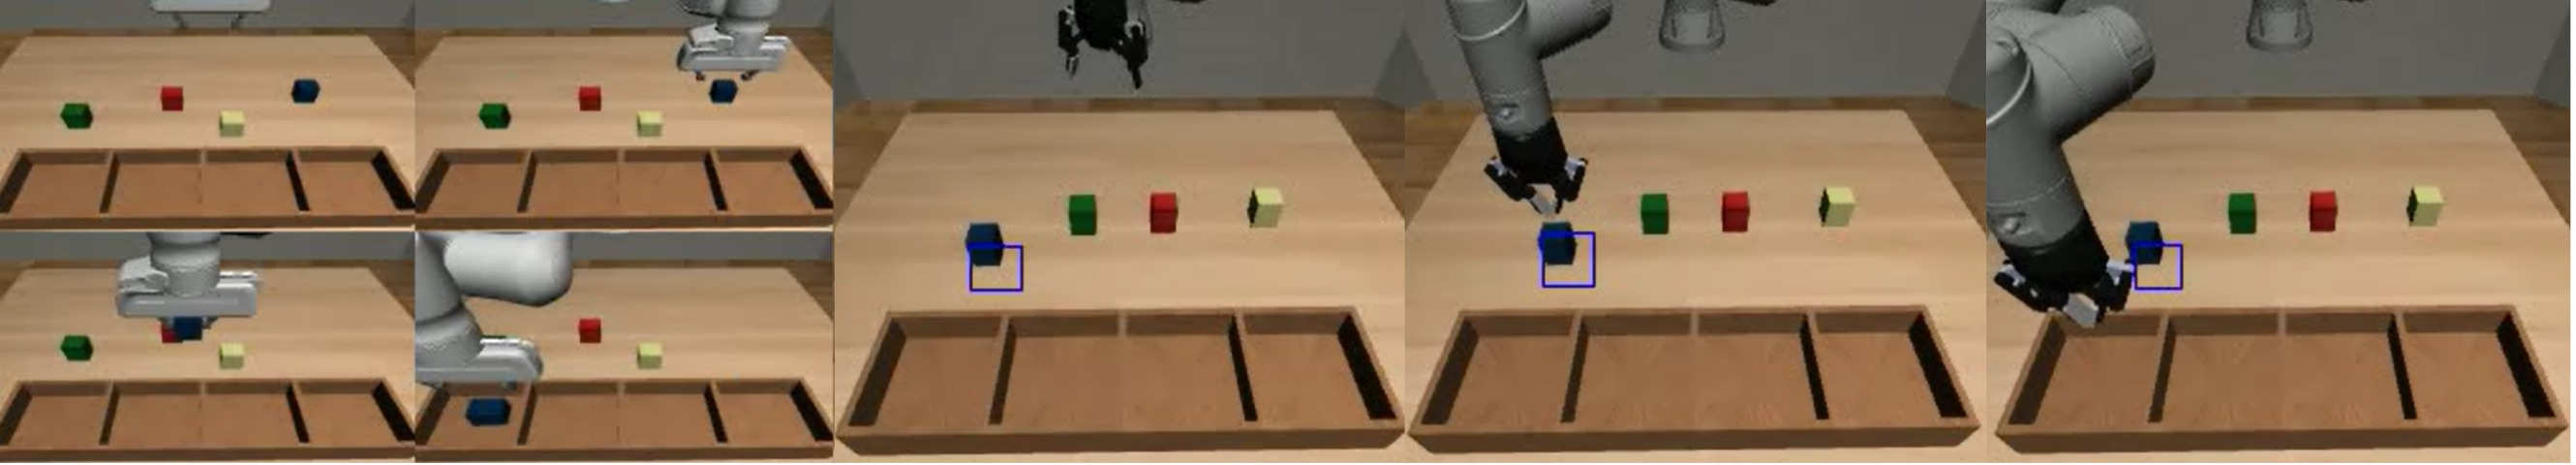
\includegraphics[width=1.0\textwidth]{figures/images/ch3/error_no_bb_after_pick.jpg}
    \caption{Example of an unsuccessful Pick-Place operation using the  ``no-bb after pick" variant. In this scenario, the robot successfully reaches the target box based on the predicted bounding box (blue). However, the single-control module prematurely predicts the closing command, preventing the robot from correctly picking up the object.}
    \label{fig:error_no_bb_after_pick}
\end{figure}

% \smalltodo{add figure}

Regarding the performance of the proposed \textit{MOSAIC-COD} module, it is notable that it achieves the highest success rate in 3 out of 4 tasks. Specifically, for tasks prone to placing the correct object in the wrong position, such as Pick-Place and Nut-Assembly, this type of error is eliminated, resulting in an overall improvement in the success rate.

Moreover, a novel variant of the MOSAIC baseline, \textit{MOSAIC-DP}, has been implemented. This model follows the classic MOSAIC architecture proposed in \cite{mandi2022towards_more_generalizable_one_shot} but is equipped with two control modules: one for the reaching primitive and another for the primitive used in the final part of the task (i.e., placing, assembly, stacking, or pushing, respectively). 

It is important to note that the performance of this variation is very similar to the original MOSAIC baseline, even though the control problem is simplified by splitting it into two phases corresponding to different primitives. Specifically, the most significant error in this case also stems from manipulating the wrong object. The success rates with the wrong object are 54.38\%, 46.67\%, 46.67\%, and 7.59\% for the Pick-Place, Nut-Assembly, Stack-Block, and Press-Button tasks, respectively. 

This further supports the central thesis, which suggests that the end-to-end architecture struggles to create an optimal embedding that addresses both cognitive and control tasks effectively.

\paragraph*{Multi-task multi-variation scenario}\mbox{}\\
\begin{table}[t]
  \scriptsize
  \selectfont
  \centering
  \refstepcounter{table}
  \caption{MOSAIC-COD results obtained in the multi-task setting. The model is compared with MOSAIC and MOSAIC-CTOD models.}
  \label{table:double_policy_multi_task}
  \resizebox{\linewidth}{!}{%
  \begin{tabular}{|c|c|c|c|c|} 
  \hline
  \textbf{Task} & \textbf{Model} & \begin{tabular}[c]{@{}c@{}}\textbf{Reaching}\\{[}\%]\end{tabular} &  \begin{tabular}[c]{@{}c@{}}\textbf{Picking}\\{[}\%]\end{tabular} & \begin{tabular}[c]{@{}c@{}}\textbf{Success}\\{[}\%]\end{tabular} \\ 
  \hhline{|=====|}
  \multirow{3}{*}{Pick-Place} & MOSAIC & 25.83$\pm$1.30 & 23.96$\pm$0.72 & 22.71$\pm$0.72 \\ 
  \cline{2-5}
   & MOSAIC-CTOD & 80.21$\pm$1.44 & 67.50$\pm$0.62 & 53.33$\pm$1.90 \\ 
  \cline{2-5}
   & \textit{MOSAIC-COD} & 100.00$\pm$0.00 & 94.79$\pm$0.90 & \textbf{89.58$\pm$3.55} \\ 
  \hhline{|=====|}
  \multirow{3}{*}{Nut-Assembly} & MOSAIC & 32.96$\pm$1.28 & 30.74$\pm$2.31 & 28.53$\pm$2.31 \\ 
  \cline{2-5}
   & MOSAIC-CTOD & 68.69$\pm$1.11 & 49.63$\pm$3.30 & 33.33$\pm$4.00 \\ 
  \cline{2-5}
   & \textit{MOSAIC-COD} & 99.63$\pm$0.64 & 78.15$\pm$2.31 & \textbf{70.74$\pm$4.49} \\ 
  \hhline{|=====|}
  \multirow{3}{*}{Stack-Block} & MOSAIC & 57.78$\pm$1.92 & 57.78$\pm$1.92 & 55.56$\pm$2.54 \\ 
  \cline{2-5}
   & MOSAIC-CTOD & 97.92$\pm$2.09 & 96.67$\pm$2.35 & \textbf{87.92$\pm$2.00} \\ 
  \cline{2-5}
   & \textit{MOSAIC-COD} & 98.33$\pm$0.00 & 98.33$\pm$0.00 & 85.00$\pm$5.00 \\ 
  \hhline{|=====|}
  \multirow{3}{*}{Press-Button} & MOSAIC & 78.33$\pm$1.66 & - & 77.22$\pm$2.54 \\ 
  \cline{2-5}
   & MOSAIC-CTOD & 92.78$\pm$0.96 & - & \textbf{91.11$\pm$2.54} \\ 
  \cline{2-5}
   & \textit{MOSAIC-COD} & 83.89$\pm$2.55 & - & 71.67$\pm$2.88 \\
  \hline
  \end{tabular}
  }
  \end{table}
Given the results and observations from the previous section, the MOSAIC-COD module is directly compared to the baselines MOSAIC and MOSAIC-CTOD in the Multi-Task setting. Table \ref{table:cod_multi_task_performance} summarizes the results. As can be seen, the use of specialized models trained for the two task phases, reaching and placing, leads to a system that consistently picks the target object. This improvement is particularly evident in the more complex tasks, such as Pick-Place and Nut-Assembly. The enhanced picking rate demonstrates that having accurate information about the target object position enables correct target acquisition, while the presence of two control modules allows for training specific controllers for simpler primitives.

However, despite the improvements observed in Pick-Place and Nut-Assembly, MOSAIC-COD has the lowest overall success rate on the Press-Button task. This can be attributed to two main factors. First, the Press-Button task is substantially different from the other three tasks. Unlike the others, it does not involve pick-and-place primitives, making it an out-of-distribution task. Second, the instability of the bounding boxes produced can lead to undesirable behaviors, such as sudden movements or freezing.
% \smalltodo{add figure}

\subsubsection{Proprioceptive state and Generalization tests}
\begin{figure}[t]
    \centering
    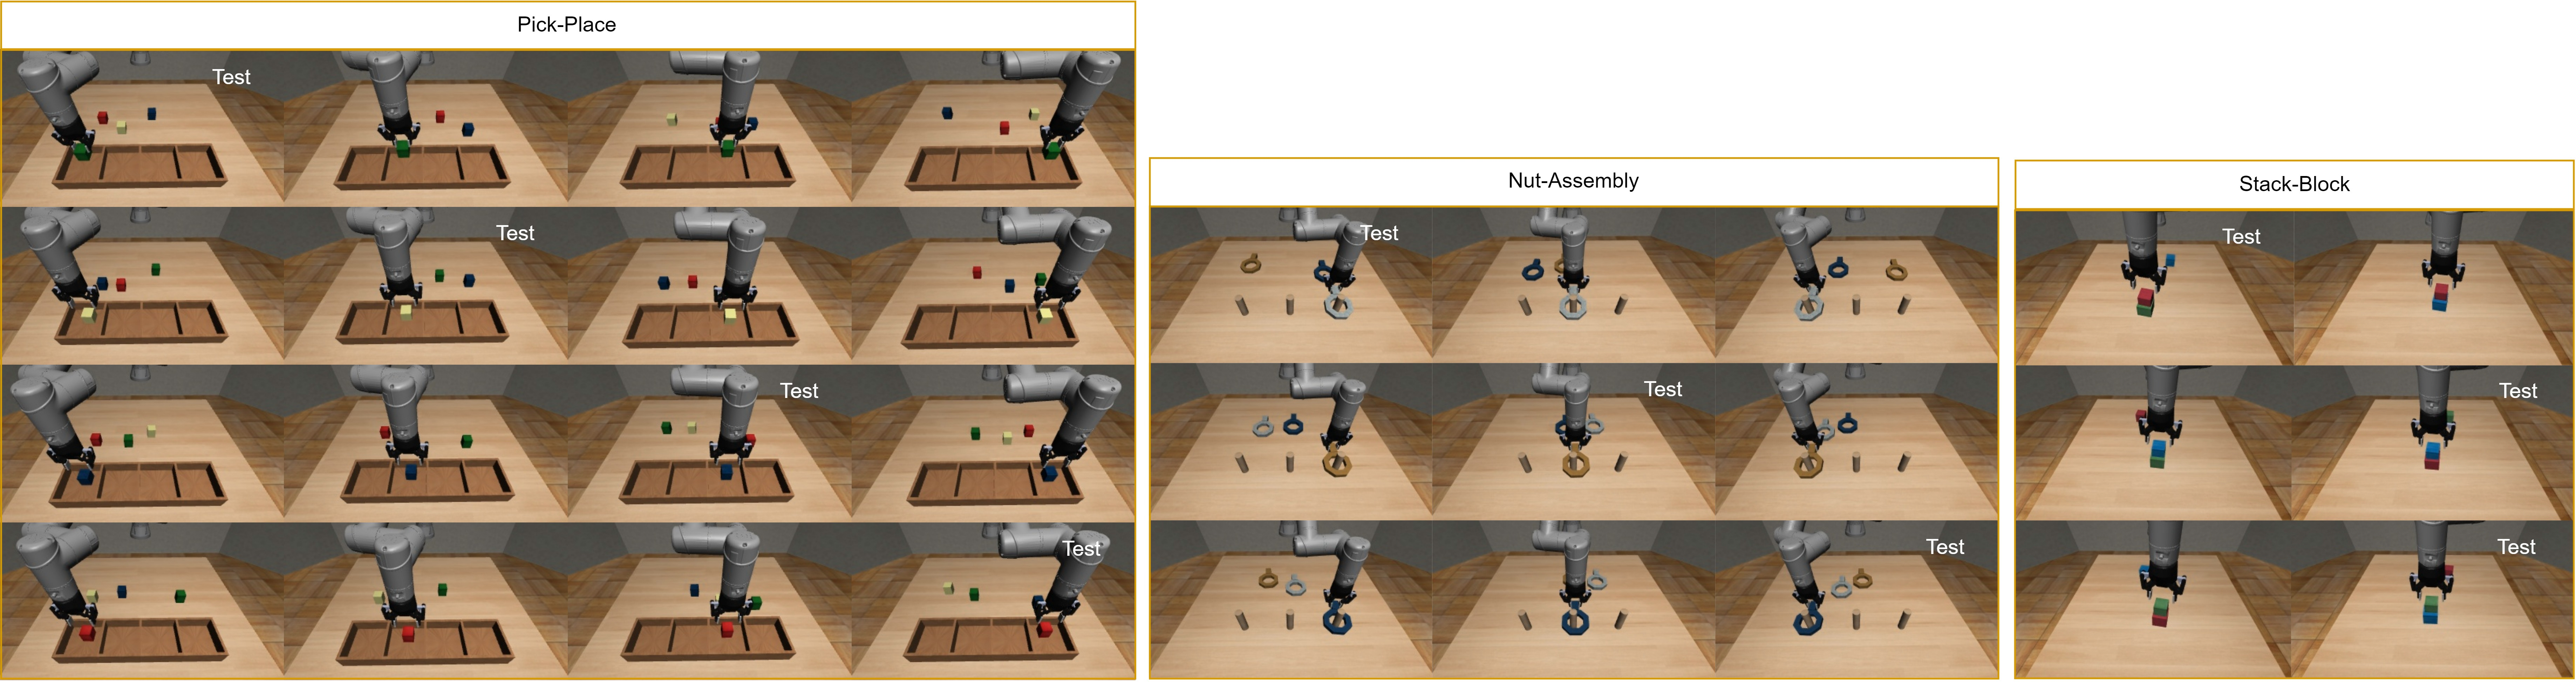
\includegraphics[width=1.0\textwidth]{figures/images/ch3/generalization_dataset.jpg}
    \caption{The dataset used for generalization tests removes one variation from each set of variations for a given target object.}
    \label{fig:generalization_dataset}
\end{figure}


\begin{figure}[t]
    \centering
    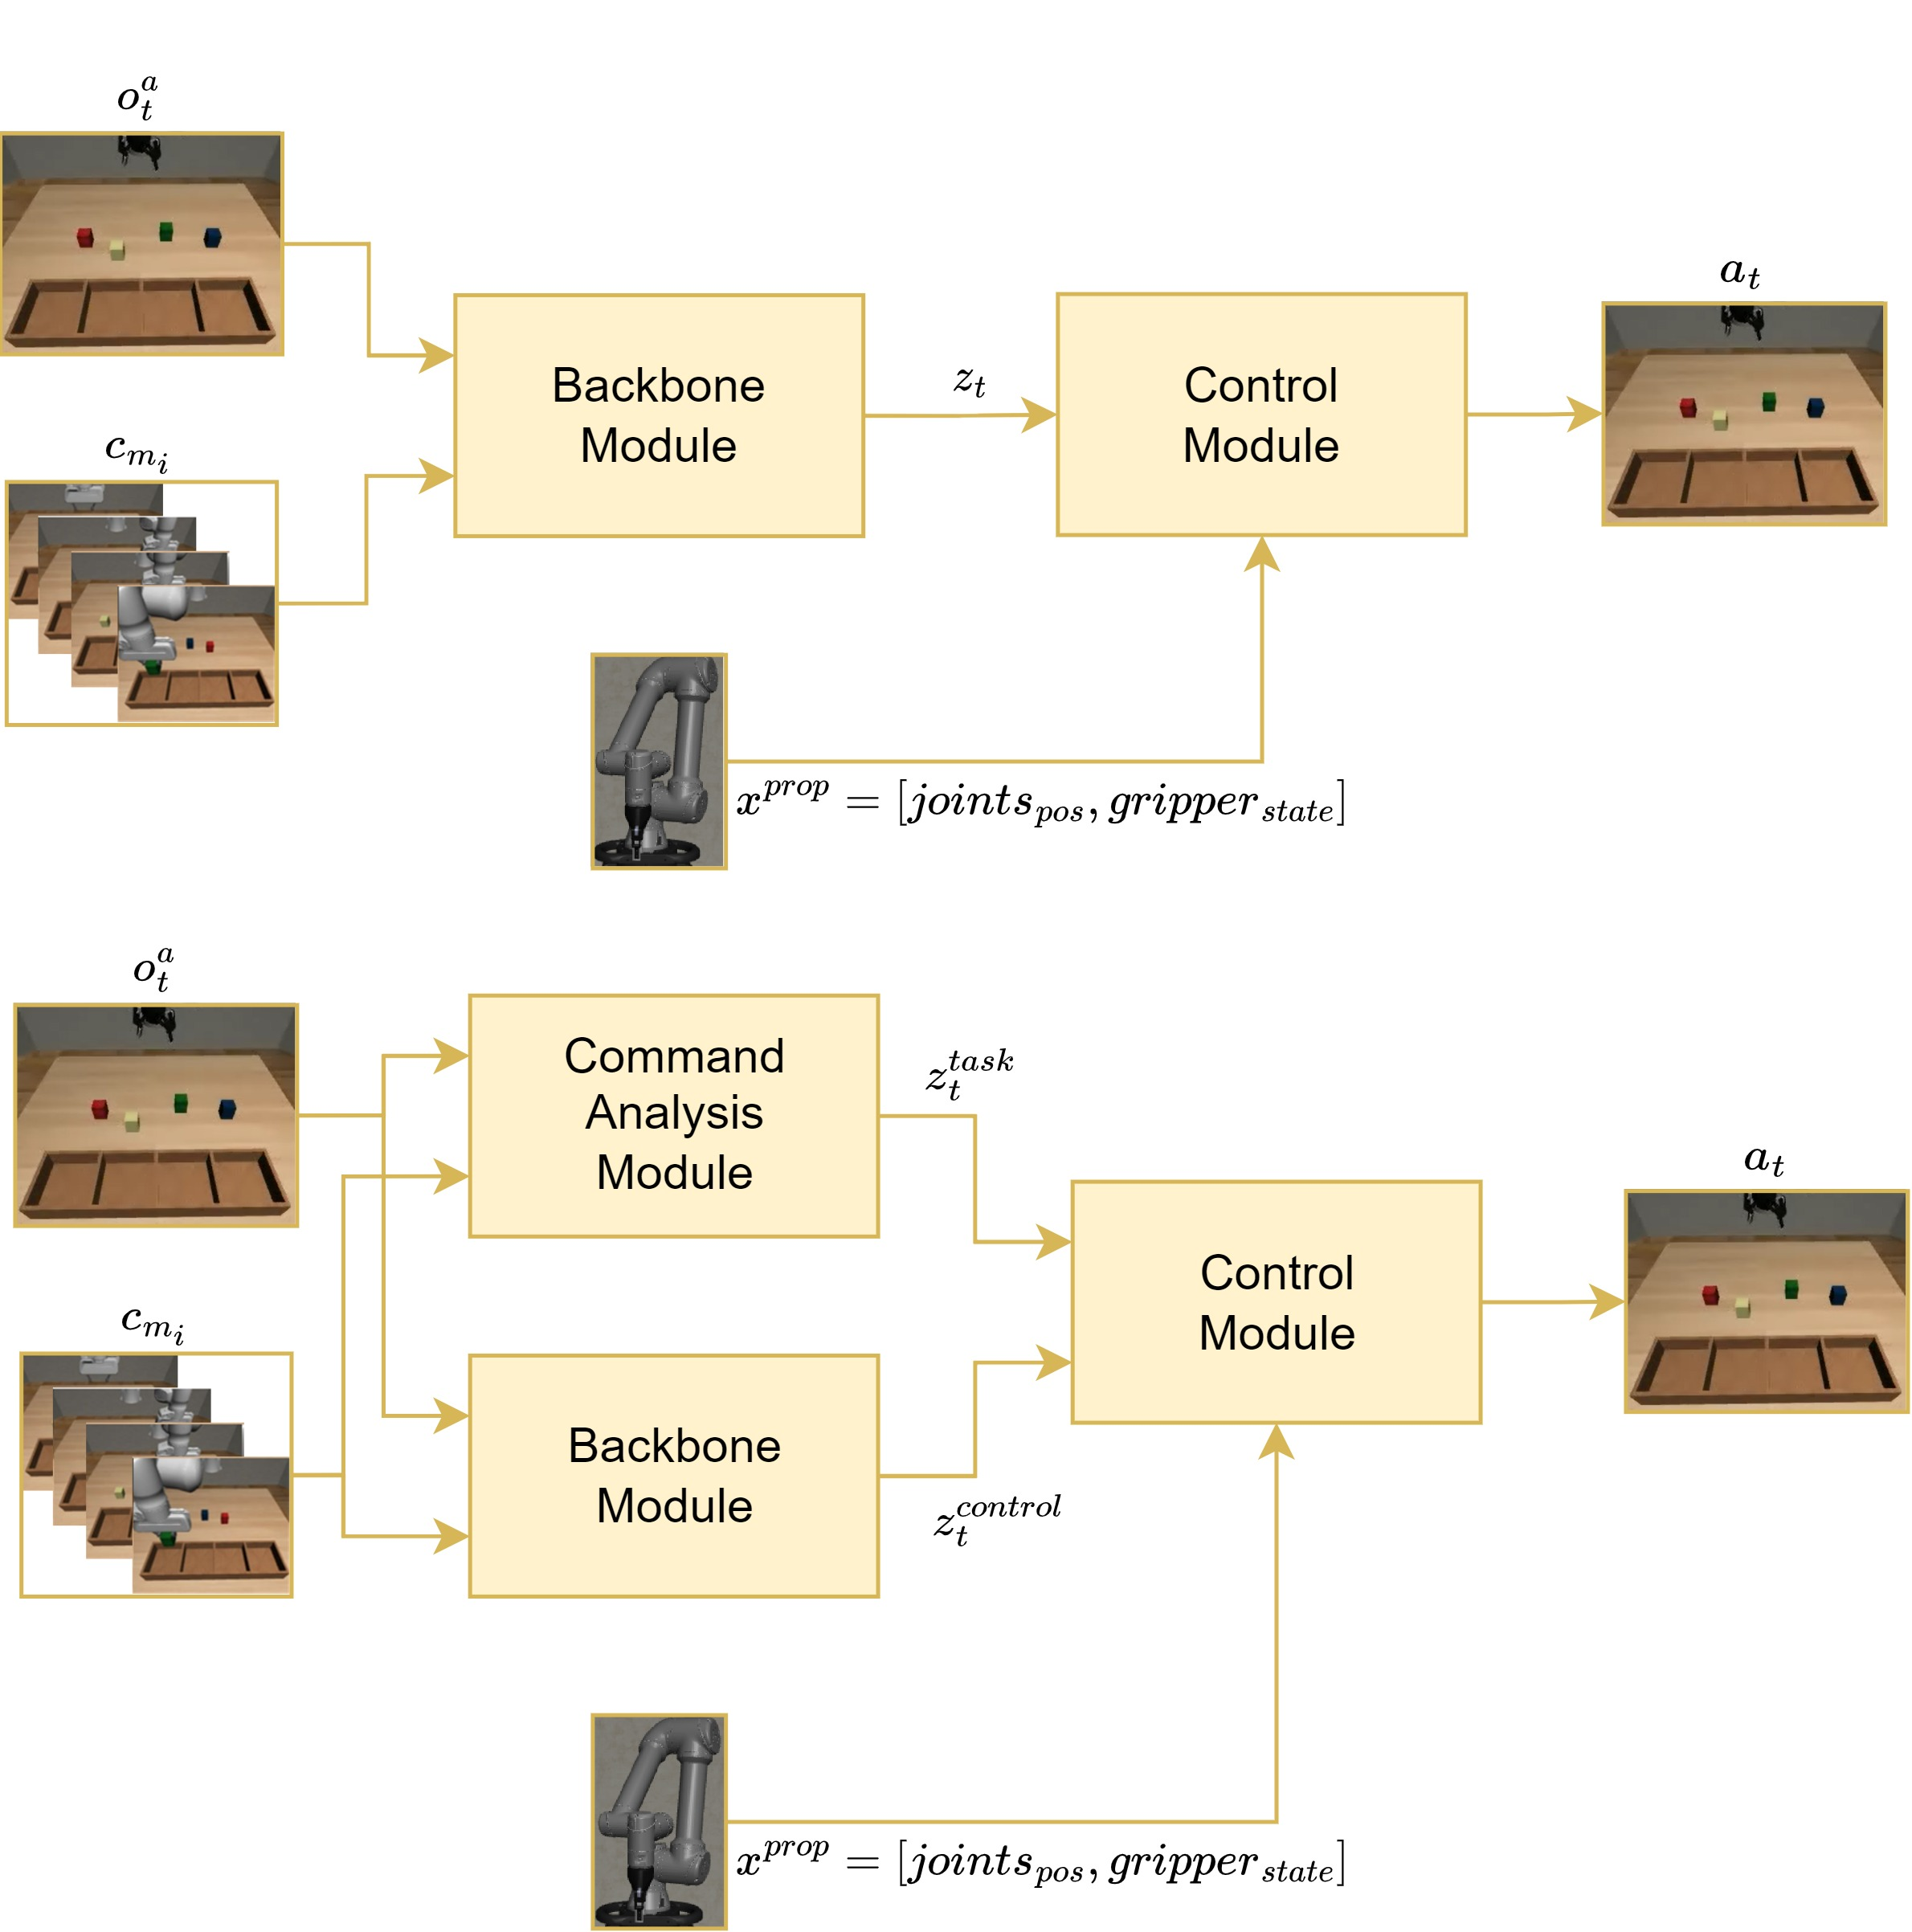
\includegraphics[width=0.7\textwidth]{figures/images/ch3/end_to_end_vs_modular_proprioceptive.jpg}
    \caption{Proprioceptive information is integrated in both the end-to-end architecture (top) and the modular architecture (bottom). The proprioceptive vector, $x^{prop}$, is constructed from the robot's six continuous joint positions and the binary gripper state.}
    \label{fig:end_to_end_vs_modular_proprioceptive}
\end{figure}

In this section, additional experiments are described, focusing on two key objectives.

The first set of experiments aims to determine whether the integration of proprioceptive information can enhance the system's robustness. This is particularly important for tasks requiring fine manipulation, such as the Nut-Assembly task, where the goal is to reduce errors during the assembly phase, specifically avoiding instances where the nut hits the peg.

The second set of experiments explores the generalization capabilities of the proposed system. Specifically, the goal is to assess whether the system can generalize to previously unseen task variations. To evaluate this, the system is trained on a subset of task variations selected as follows: for a set of variations involving a specific target object (e.g., a green box), one variation is excluded (e.g., placing the box into the first bin). However, in other sets involving different objects, the variation that requires placing the object into the first bin is retained. This setup allows for testing how well the system can transfer knowledge across different variations. By doing so, it becomes possible to evaluate whether the system can achieve robust performance with less training data, eliminating the need to collect every possible variation for each object (Figure \ref{fig:generalization_dataset}).
% \smalltodo{add figure}

\begin{table}[t]
  \centering
  \caption{The results obtained by integrating proprioceptive information in both Single-Task and Multi-Task scenarios. For each baseline model, MOSAIC, MOSAIC-CTOD, and MOSAIC-COD, the corresponding version that includes the proprioceptive state (P) was trained and tested.}
  \label{table:proprioceptive}
  \resizebox{\linewidth}{!}{%
  \begin{tabular}{|c|c|c|c|} 
  \hline
  \textbf{Task} & \textbf{Model} & \begin{tabular}[c]{@{}c@{}}\textbf{Success}\\\textbf{(Single-Task)}\\{[}\%]\end{tabular} & \begin{tabular}[c]{@{}c@{}}\textbf{Success}\\\textbf{(Multi-Task)}\\{[}\%]\end{tabular} \\ 
  \hhline{|====|}
  \multirow{6}{*}{Pick-Place} & MOSAIC & 58.75$\pm$1.87 &  \\ 
  \cline{2-4}
   & \textit{MOSAIC-P} & 12.84$\pm$0.31 &  \\ 
  \cline{2-4}
   & MOSAIC-CTOD & 77.11$\pm$5.60 &  \\ 
  \cline{2-4}
   & \textit{MOSAIC-CTOD-P} & 87.84$\pm$2.43 &  \\ 
  \cline{2-4}
   & MOSAIC-COD & 93.33$\pm$0.72 &  \\ 
  \cline{2-4}
   & \textit{MOSAIC-COD-P} & \textbf{96.04$\pm$0.56} &  \\ 
  \hhline{|====|}
  \multirow{6}{*}{Nut-Assembly} & MOSAIC & 33.33$\pm$1.11 &  \\ 
  \cline{2-4}
   & \textit{MOSAIC-P} & 13.83$\pm$0.57 &  \\ 
  \cline{2-4}
   & MOSAIC-CTOD & 64.07$\pm$0.64 &  \\ 
  \cline{2-4}
   & \textit{MOSAIC-CTOD-P} & 95.06$\pm$0.56 &  \\ 
  \cline{2-4}
   & MOSAIC-COD & 81.11$\pm$3.84 &  \\ 
  \cline{2-4}
   & \textit{MOSAIC-COD-P} & \textbf{95.06$\pm$0.57} &  \\ 
  \hhline{|====|}
  \multirow{6}{*}{Stack-Block} & MOSAIC & 53.33$\pm$1.66 &  \\ 
  \cline{2-4}
   & \textit{MOSAIC-P} & 29.07$\pm$2.50 &  \\ 
  \cline{2-4}
   & MOSAIC-CTOD & 91.67$\pm$2.88 &  \\ 
  \cline{2-4}
   & \textit{MOSAIC-CTOD-P} & 91.11$\pm$6.90 &  \\ 
  \cline{2-4}
   & \textit{MOSAIC-COD} & 95.00$\pm$1.66 &  \\ 
  \cline{2-4}
   & \textit{MOSAIC-COD-P} & \textbf{96.67$\pm$1.66} &  \\ 
  \hhline{|====|}
  \multirow{6}{*}{Press-Button} & MOSAIC & \textbf{100.00$\pm$0.00} &  \\ 
  \cline{2-4}
   & \textit{MOSAIC-P} & 65.00$\pm$3.33 &  \\ 
  \cline{2-4}
   & MOSAIC-CTOD & 95.56$\pm$1.92 &  \\ 
  \cline{2-4}
   & \textit{MOSAIC-CTOD-P} & 86.66$\pm$6.66 &  \\ 
  \cline{2-4}
   & MOSAIC-COD & 91.11$\pm$1.92 &  \\ 
  \cline{2-4}
   & \textit{MOSAIC-COD-P} & 72.03$\pm$3.39 &  \\
  \hline
  \end{tabular}
  }
  \end{table}
\paragraph*{Proprioceptive information}\mbox{}\\
The proprioceptive information selected for the four tasks considered includes the joint positions, $joints_{pos} \in \mathcal{R}^{6}$ and the gripper state, $gripper_{state} \in \left[ 0, 1 \right]$. This vector of elements, $x^{prop}$, is provided as input directly to the Control Module, as shown in Figure \ref{fig:end_to_end_vs_modular_proprioceptive}. 
% \smalltodo{add figure}

Specifically, for each baseline method, \textit{MOSAIC}, \textit{MOSAIC-CTOD}, and \textit{MOSAIC-COD}, a version of the model incorporating proprioceptive information was trained. Table \ref{table:proprioceptive} presents the success rates for both the Single-Task and Multi-Task scenarios. 

It is important to note that for 3 out of 4 tasks, the best performance is achieved by combining the Double-Policy approach with proprioceptive information, effectively solving the manipulation tasks of Pick-Place, Nut-Assembly, and Stack-Block in a robust manner. The greatest improvement is seen in the Nut-Assembly task, where the proprioceptive information resolves issues related to collisions and robot freezing.

However, this improvement is not observed in the Press-Button task, where a 35\% drop in success rate is seen, even with the \textit{MOSAIC} baseline. In this task, the main failure cases are related to unstable robot behavior. Additionally, in variations focused on object orientation, the robot often gets stuck when correctly approaching the button.

Notably, the same behavior is not observed in the Multi-Task scenario. In fact, the highest performance is achieved by methods that exclude proprioceptive information. Specifically, the introduction of proprioceptive data appears to exacerbate the imbalance between tasks, hindering the system from effectively utilizing this additional information during testing, which leads to instability. 

For example, in the case of the MOSAIC-CTOD-P module, the robot successfully picks the target object only 58.87\% of the time. This occurs because the closing command is sent too early, relative to the object position. Furthermore, the success rate drops further to 38.14\%, as the robot, despite reaching the target peg, collides with it, an issue where proprioceptive information should theoretically provide assistance, especially since the pegs are fixed.

This instability is most evident in the Stack-Block task, where the success rate falls to 22.77\% for the MOSAIC-COD-P module, despite the robot picking the target object with an average rate of 80.00\%. The errors in this case are due to the object being dropped during stacking, caused by imprecise placement, as well as instances where the robot becomes completely stuck.

These results highlight the need for a balanced learning procedure in the context of Multi-Task Learning, as discussed earlier in Section \ref{sec:ocpl_results_scm}.

% \usepackage{graphicx}
% \usepackage{multirow}
% \usepackage{hhline}


\begin{table}[t]
  \centering
  \caption{The results obtained by testing the models on unseen variations.}
  \label{table:generalization}
  \resizebox{\linewidth}{!}{%
  \begin{tabular}{|c|c|c|c|c|c|} 
  \hline
  \textbf{Task} & \textbf{Model} & \begin{tabular}[c]{@{}c@{}}\textbf{Reaching}\\\textbf{(Single-Task)}\\{[}\%]\end{tabular} & \begin{tabular}[c]{@{}c@{}}\textbf{Success}\\\textbf{(Single-Task)}\\{[}\%]\end{tabular} & \begin{tabular}[c]{@{}c@{}}\textbf{Reaching}\\\textbf{(Multi-Task)}\\{[}\%]\end{tabular} & \begin{tabular}[c]{@{}c@{}}\textbf{Success}\\\textbf{(Multi-Task)}\\\textbf{\textbf{}}\%]\end{tabular} \\ 
  \hhline{|======|}
  \multirow{3}{*}{\vspace{-30px}\rotatebox[origin=c]{90}{Pick-Place}} & MOSAIC & 35.83$\pm$2.82 & 31.67$\pm$3.82 & 32.50$\pm$2.50 & 20.83$\pm$5.70 \\ 
  \cline{2-6}
   & \begin{tabular}[c]{@{}c@{}}\textbf{\textit{MOSAIC-CTOD}}\\\textbf{\textit{(proposal)}}\end{tabular} & 100.00$\pm$0.00 & 87.50$\pm$4.30 & 100.00$\pm$0.00 & 63.33$\pm$5.20 \\ 
  \cline{2-6}
   & \begin{tabular}[c]{@{}c@{}}\textbf{\textit{MOSAIC-COD}}\\\textbf{\textit{(proposal)}}\end{tabular} & 100.00$\pm$0.00 & \textbf{89.17$\pm$2.89} & 100.00$\pm$0.00 & \textbf{94.17$\pm$2.88} \\ 
  \hhline{|======|}
  \multirow{3}{*}{\vspace{-30px}\rotatebox[origin=c]{90}{Nut-Assembly}} & MOSAIC & 22.22$\pm$1.93 & 13.33$\pm$3.33 & 27.78$\pm$3.85 & 18.88$\pm$3.84 \\ 
  \cline{2-6}
   & \begin{tabular}[c]{@{}c@{}}\textbf{\textit{MOSAIC-CTOD}}\\\textbf{\textit{(proposal)}}\end{tabular} & 100.00$\pm$0.00 & 38.89$\pm$6.94 & 100.00$\pm$0.00 & 51.11$\pm$1.92 \\ 
  \cline{2-6}
   & \begin{tabular}[c]{@{}c@{}}\textbf{\textit{MOSAIC-COD}}\\\textbf{\textit{(proposal)}}\end{tabular} & 98.89$\pm$1.93 & \textbf{57.78$\pm$5.09} & 100.00$\pm$0.00 & \textbf{90.00$\pm$3.33} \\ 
  \hhline{|======|}
  \multirow{3}{*}{\vspace{-30px}\rotatebox[origin=c]{90}{Stack-Block}} & MOSAIC & 58.89$\pm$1.93 & 53.33$\pm$3.33 & 60.00$\pm$5.77 & 56.66$\pm$3.33 \\ 
  \cline{2-6}
   & \begin{tabular}[c]{@{}c@{}}\textbf{\textit{MOSAIC-CTOD}}\\\textbf{\textit{(proposal)}}\end{tabular} & 100.00$\pm$0.00 & 94.44$\pm$6.94 & 100.00$\pm$0.00 & \textbf{88.88$\pm$5.00} \\ 
  \cline{2-6}
   & \begin{tabular}[c]{@{}c@{}}\textbf{\textit{MOSAIC-COD}}\\\textbf{\textit{(proposal)}}\end{tabular} & 100.00$\pm$0.00 & \textbf{97.78$\pm$1.93} & 100.00$\pm$0.00 & 72.20$\pm$5.09 \\
  \hline
  \end{tabular}
  }
  \end{table}
\paragraph*{Generalization}\mbox{}\\
Regarding the generalization tests, we evaluated only the three tasks where the previously explained variation selection was applicable. Specifically, the following variations were removed for each task (Figure \ref{fig:generalization_dataset}):

\begin{itemize}
    \item \textbf{Pick-Place}: Variations 1, 6, 11, and 16 were excluded.
    \item \textbf{Nut-Assembly}: Variations 1, 5, and 9 were excluded.
    \item \textbf{Stack-Block}: Variations 1, 4, and 6 were excluded.
\end{itemize}

The models were trained on the remaining variations and tested on the excluded ones following the same procedure.

Table \ref{table:generalization} summarizes the success rates obtained for both the Single-Task and Multi-Task settings. Notably, with the introduction of the CTOD and COD modules, the system consistently reaches the correct target object in unseen variations. Similarly, the robot is able to pick and complete tasks, outperforming the MOSAIC baseline across all tested tasks.

This is a promising result, as it demonstrates that the system can effectively share knowledge across different variations, enabling robust training with fewer data.


